\documentclass[a4paper,10pt]{article}

\usepackage{amsmath}
\usepackage{amstext}
\usepackage{amssymb}
\usepackage{amsfonts}
\usepackage{amsthm}
\usepackage{etoolbox}
%mathspec/fontspec
\usepackage{mathspec}
\usepackage{xunicode}
\usepackage{xltxtra}

\usepackage[bookmarks,bookmarksnumbered]{hyperref}

\makeatletter       % changes [1] to 1. in bibliography
\renewcommand{\@biblabel}[1]{#1.}
\makeatother

\usepackage{appendix}
\usepackage{graphicx}
\usepackage{natbib}


% FONT
\setmainfont[Mapping=tex-text,Numbers={Lining}]{Linux Libertine O}
\setmathfont(Latin)[Numbers={Lowercase}]{Linux Libertine O}
\setmathfont(Digits)[Scale=MatchLowercase]{Linux Libertine O}

\usepackage{unicode-math}
\setmainfont[Mapping=tex-text,Numbers={Lining}]{Linux Libertine O} 
\setmathfont{XITS Math}

\setmathfont[range={\mathup}]{Linux Libertine O} 
\setmathfont[range={\mathit}]{Linux Libertine O Italic} 
\setmathfont[range={\rm}]{Linux Libertine O} 
\setmathfont[range={\mathrm}]{Linux Libertine O} 



% \renewcommand{\rmdefault}{fxl}
\renewcommand{\sfdefault}{txss}


%%%%%%%%% from here yuasa setting %%%%%%%%%%%%%%%%%%%%%
% a4paper paperheight = 845.04684pt
%\setlength{\topmargin}{-.5in}
%% textheight = paperheight - 2in - \topmargin - \headheight - \headsep
%%              - \footskip = approx. 641pt
%\setlength{\textheight}{1.05\paperheight}
%\addtolength{\textheight}{-2.2in}
%%\addtolength{\textheight}{-\topmargin}
%%\addtolength{\textheight}{-\headheight}
%%\addtolength{\textheight}{-\headsep}
%%\addtolength{\textheight}{-\footskip}

%% a4paper paperwidth = 597.50787pt
%%\setlength{\marginparsep}{0pt}
%%\setlength{\marginparwidth}{0pt}
%% textwidth = paperwidth - 2in - \oddsidemargin = approx. 432pt
%\setlength{\textwidth}{\paperwidth}
%\addtolength{\textwidth}{-1.8in}
%%\addtolength{\textwidth}{-\oddsidemargin}

%% add 20pt to sidemargin
%%   oddside: 1in+20pt+20pt | \textwidth | 1in-20pt
%%   evenside: 1in-20pt | \textwidth | 1in+20pt+20pt
%\setlength{\oddsidemargin}{0pt}
%\setlength{\evensidemargin}{0pt}

%%%%%%%%% to here yuasa setting %%%%%%%%%%%%%%%%

%%%%%%%%% from here margin setting %%%%%%%%%%%%%%%%
%for dron
%\setlength{\topmargin}{0pt}
%\setlength{\marginparsep}{0pt}
%\setlength{\marginparwidth}{0pt}
%\setlength{\oddsidemargin}{20pt}
%\setlength{\evensidemargin}{0pt}
%
%\setlength{\textwidth}{\paperwidth}
%\addtolength{\textwidth}{-2in}
%\addtolength{\textwidth}{-\oddsidemargin}
%
%\addtolength{\oddsidemargin}{0pt}
%\addtolength{\evensidemargin}{-23pt}
%\setlength{\topmargin}{-12mm}
%\setlength{\textheight}{25.3cm}
%\setlength{\textwidth}{16.3cm}
%%%%%%%%% till here margin setting %%%%%%%%%%%%%%%%

%%% Linestrech
%for user guide
\renewcommand{\baselinestretch} {1.1}
%for dron
%\renewcommand{\baselinestretch} {1.1}

\setlength\bibsep{2pt}
\renewcommand{\bibnumfmt}[1]{(#1)}


%%% Table of Contents
\usepackage{tocloft}
\setlength\cftparskip{-0.7pt}
\setlength\cftbeforesecskip{1.5pt}
\setlength\cftaftertoctitleskip{2pt}

\addtolength{\oddsidemargin}{-.875in}
	\addtolength{\evensidemargin}{-.875in}
	\addtolength{\textwidth}{1.75in}

	\addtolength{\topmargin}{-.875in}
	\addtolength{\textheight}{1.75in}

%% for quotes
%\fontspec[Mapping=tex-text]{Linux Libertine O}
%\fontspec[Ligatures=TeX]{Linux Libertine O}

%%%%%%%%% color %%%%%%%%%
\usepackage{color}
\newcommand{\red}{\textcolor{red}}
\newcommand{\green}{\textcolor{green}}
\newcommand{\blue}{\textcolor[rgb]{0,0,0.8}}
\newcommand{\midnightblue}{\textcolor[rgb]{0.0976,0.0976,0.4375}}
\newcommand{\apricot}{\textcolor[rgb]{1,0,0.5}}
\newcommand{\strawberry}{\textcolor[rgb]{1,0,0.5}}
\newcommand{\orange}{\textcolor[rgb]{0.949, 0.593, 0}}
\newcommand{\gray}{\textcolor[rgb]{0.4,0.4,0.4}}
%%%%%%%%%%%%%%%%%%%%%%%%%%%


%%%%%%%%% for source code listing %%%%%%%%%
\usepackage{listings}


\lstset{%
 language={XML},
 backgroundcolor={\color[gray]{.97}},%
 basicstyle={\small\ttfamily},%
% identifierstyle={\small\ttfamily},%
 commentstyle={\gray},%
% keywordstyle={\small\bfseries\ttfamily},%
% ndkeywordstyle={\small},%
% stringstyle={\apricot},
 frame={tb},
 breaklines=true,
% columns=[l]{fullflexible},%
 numbers=left,%
% xrightmargin=5pt,%
% xleftmargin=5pt,%
% numberstyle={\scriptsize},%
% stepnumber=1,
 numbersep=5pt,%
 lineskip=-0.5pt,%
 showstringspaces=false,
 numbers=none
}
%%%%%%%%%%%%%%%%%%%%%%%%%%%

\title{\Huge{
SpaceWire RMAP GUI}\\
\Large{User Guide}}

\author{
{\Large
Takayuki Yuasa
}\\
{\small Japan Aerospace Exploration Agency, Institute of Space and Astronautical Science}\\
{\small yuasa \_at\_mark\_ astro.isas.jaxa.jp}\\
}

\date{January 11, 2012}

%\newcommand{\red}{\textcolor{red}}
%\newcommand{\green}{\textcolor{green}}
%\newcommand{\blue}{\textcolor{blue}}
%\newcommand{\apricot}{\textcolor[rgb]{1,0,0.5}}

\usepackage{listings}
\usepackage{color}

\lstset{%
 language={XML},
 backgroundcolor={\color[gray]{.97}},%
 basicstyle={\small\ttfamily},%
 identifierstyle={\small\ttfamily},%
 commentstyle={\small\ttfamily\itshape},%
 keywordstyle={\small\bfseries\ttfamily},%
 ndkeywordstyle={\small},%
 stringstyle={\small\ttfamily\apricot},
 frame={tb},
 breaklines=true,
% columns=[l]{fullflexible},%
 numbers=left,%
 xrightmargin=5pt,%
 xleftmargin=5pt,%
% numberstyle={\scriptsize},%
% stepnumber=1,
 numbersep=5pt,%
 lineskip=-0.5pt%
}

\begin{document}
\maketitle
\tableofcontents

\setcounter{page}{2}

%%%%%%%%%%%%%%%%%%%%%%%%%%%%%%%%%%%%%%
%%%%%%%%%%%%%%%%%%%%%%%%%%%%%%%%%%%%%%
\section{Overview of SpaceWire RMAP GUI}
SpaceWire RMAP GUI is an easy-to-use graphical user interface front end for SpaceWire-to-GigabitEther. The software runs on Mac OS X, and is capable of sending and receiving raw SpaceWire packets, and performing RMAP\footnote{Remote Memory Access Protocol.} read/write transactions using a SpaceWire interface connected to your Mac. SpaceWire-to-GigabitEther is a default SpaceWire interface supported by SpaceWire RMAP GUI. 
In addition to these, RMAP packet construction/interpretation is provided. The software is developed as an open-source project, and contributions and/or feedbacks from users or developers are highly appreciated.

Several types of information used in SpaceWire RMAP GUI, such as RMAP target node information, memory object on an RMAP target node, can be defined using XML-like file. By loading definition files, users do not need to input logical address, target SpaceWire address, memory address, length, or other properties every RMAP access.

\subsection{Screenshot}
As shown in Figure \ref{figure:tab_rmap}, the main window consists of three tabs which displays SpaceWire, RMAP, and RMAP packet utility functionalities.
\begin{figure}[htb]
\begin{center}
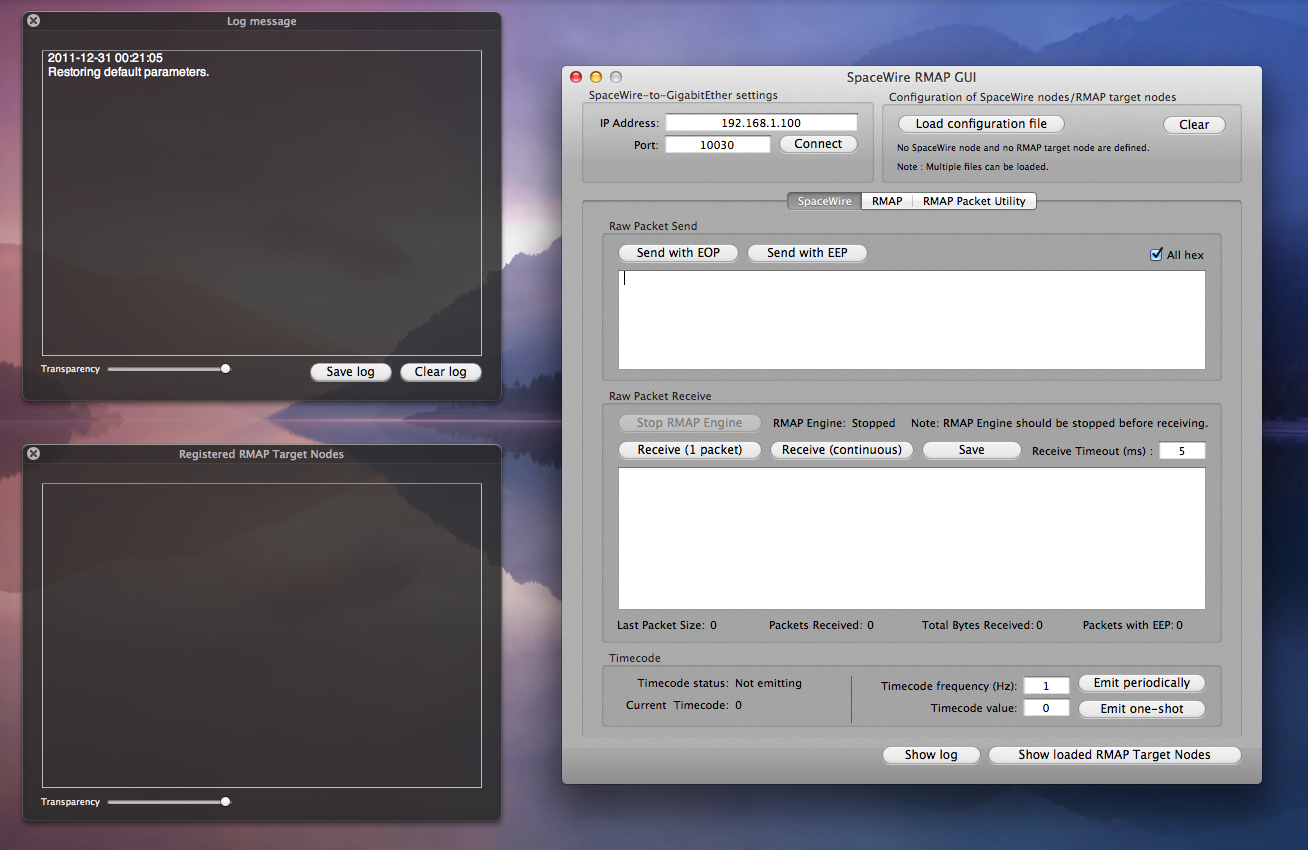
\includegraphics[width=15cm]{figures/SpaceWireRMAPGUI/Screenshot_all.png}
\caption{Screenshot of SpaceWire RMAP GUI.}
\label{figure:tab_rmap}
\end{center}
\end{figure}

\subsection{Dependence}
SpaceWire RMAP GUI uses libraries listed below:
\begin{itemize}
  \setlength{\parskip}{0cm}
  \setlength{\itemsep}{0cm}
\item SpaceWire/RMAP Library\footnote{\url{https://github.com/yuasatakayuki/SpaceWireRMAPLibrary}}
\item CxxUtilities\footnote{\url{https://github.com/yuasatakayuki/CxxUtilities}}
\item XMLUtility by Soki Sakurai from The University of Tokyo\footnote{\url{https://github.com/sakuraisoki/XMLUtilities/}}
\item xerces-c++ by the Apache project\footnote{\url{http://xerces.apache.org/xerces-c/}}
\end{itemize}
These libraries are statically linked to the software, and therefore, users are not required to install individual libraries separately.

\subsection{Download, install, and updates}
SpaceWire RMAP GUI can be downloaded from the Open-source SpaceWire project$^\mathrm{\ref{url:supportpage}}$.
Note that the software is distributed for free assuming that this is useful for some users without any warranty.
Unzip the archive, and move the extracted "SpaceWire RMAP GUI" folder to the "Applications" folder.
If you use the software frequently, register it to the Dock by dragging-and-dropping the icon to the Dock. To uninstall the software, move the "SpaceWire RMAP GUI" folder to the Trash.

Hopefully, SpaceWire RMAP GUI will be updated based on feedbacks from users, and new versions will be available at the same web site. At this moment, there is no auto update function in the software, and therefore, please check the web site for updates occasionally.


%%%%%%%%%%%%%%%%%%%%%%%%%%%%%%%%%%%%%%
%%%%%%%%%%%%%%%%%%%%%%%%%%%%%%%%%%%%%%
\section{About this user guide}
The user guide is provided {\it as is} expecting that this is somewhat useful for users to use the software. This is a voluntary mission, and therefore, kind help is always welcome. It is greatly appreciated to make contributions by feed-backing comments, revising documents, and so on.

\subsection{Latest information and feedback}
Latest information on SpaceWire RMAP GUI and SpaceWire-to-GigabitEther can be found at the open-source SpaceWire project website \footnote{The open-source SpaceWire project: \url{https://galaxy.astro.isas.jaxa.jp/~yuasa/SpaceWire}\label{url:supportpage}}.

\subsection{References}
Documents listed below can be a nice reference when better understanding SpaceWire RMAP GUI. Some of the documents can be obtained from the open-source SpaceWire project website$^\mathrm{\ref{url:supportpage}}$.
\begin{itemize}
  \setlength{\parskip}{0cm}
  \setlength{\itemsep}{0cm}
\item SpaceWire/RMAP Library User Guide
\item SpaceWire-to-GigabitEther User Guide
\item ECSS-E-ST-50-12C - "SpaceWire - Links, nodes, routers and networks" by ECSS
\item ECSS-E-ST-50-52C "SpaceWire - Remote memory access protocol" by ECSS
\end{itemize}

\subsection{Revisions}
\begin{itemize}
  \setlength{\parskip}{0cm}
  \setlength{\itemsep}{0cm}
\item 2012-01-11 Takayuki Yuasa. Typo fixed. RMAP CRC calculator was added.
\item 2012-01-06 Takayuki Yuasa. First release.
\end{itemize}



%%%%%%%%%%%%%%%%%%%%%%%%%%%%%%%%%%%%%%
%%%%%%%%%%%%%%%%%%%%%%%%%%%%%%%%%%%%%%
\section{Structure of SpaceWire RMAP GUI}

\subsection{The main window}
SpaceWire RMAP GUI displays single main window when start up.
The window contains three tabs (or panels), and each tab collects text fields and buttons which are necessary for SpaceWire, RMAP, and RMAP Packet Utility functions.

The main window is divided into four sections; the SpaceWire-to-GigabitEther setting section (top left; see Section \ref{section:setting_section}), the configuration file section (top right; see Section \ref{section:configuration_section}), the main tab (middle), and the log message section (bottom). When the main window is closed, SpaceWire RMAP GUI quits. If SpaceWire-to-GigabitEther is connected via TCP/IP when quitting, SpaceWire RMAP GUI tries to close the connection. Settings (values contained in each input fields) are saved to the preference file, and loaded again at the start up.

\subsection{SpaceWire tab}
Figure \ref{figure:SpaceWireTab} shows the SpaceWire tab.
Receive timeout can be manually set.
The tab allows users to send and receive raw SpaceWire packets.
Periodic or ordered timecode emission is managed from this tab as well.

\begin{figure}[htb]
\begin{center}
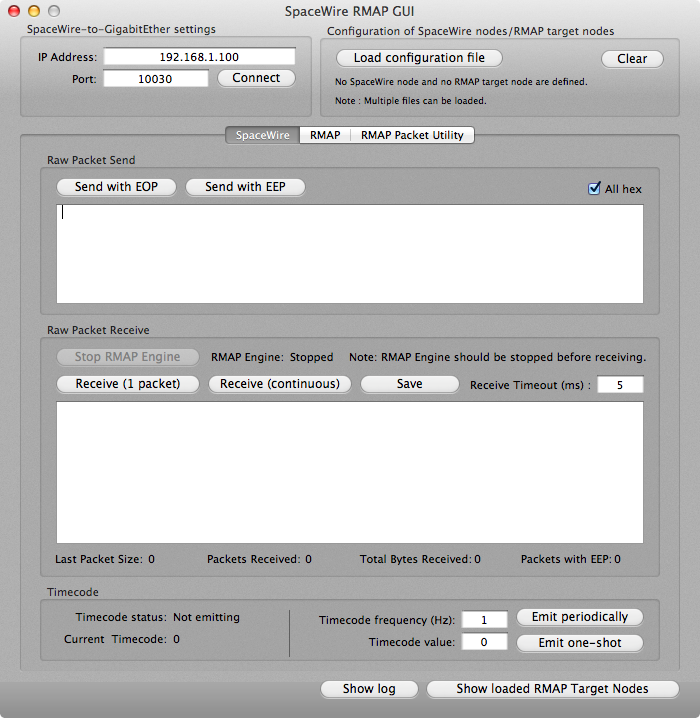
\includegraphics[width=8cm]{figures/SpaceWireRMAPGUI/Screenshot_SpaceWireTab.png}
\caption{Screenshot of the SpaceWire tab.}
\label{figure:SpaceWireTab}
\end{center}
\end{figure}

\subsection{RMAP tab}
The RMAP tab provides RMAP read/write initiator functions as shown in Figure \ref{figure:RMAPTab}.
RMAP target node information can be set manually or semi-automatically using XML-like configuration files.


\subsection{RMAP Packet Utility tab}
The RMAP Packet Utility tab, shown in Figure \ref{figure:RMAPPacketUtilityTab}, interprets and constructs RMAP packets.
A correct header or data CRC value is displayed when interpreting a packet with an invalid CRC.

\begin{figure}[htb]
\begin{center}
\begin{minipage}{0.45\hsize}
\begin{center}
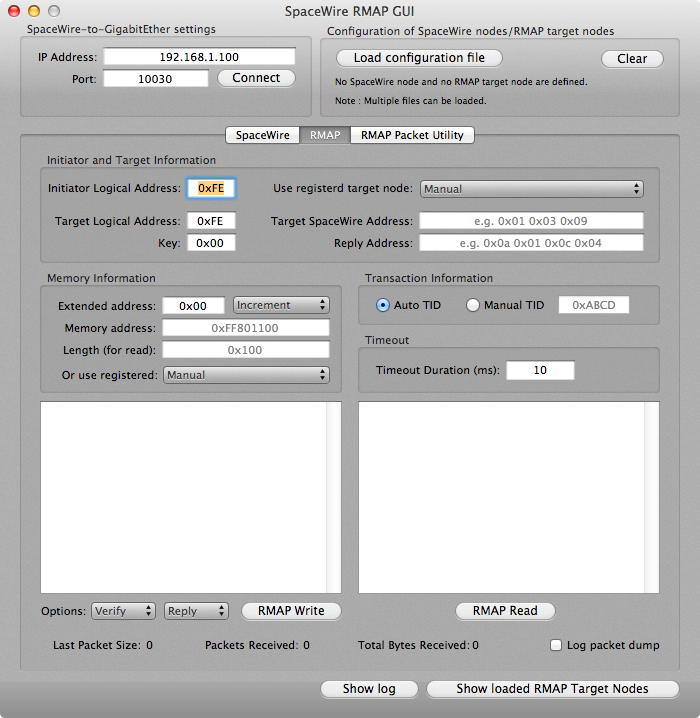
\includegraphics[width=8cm]{figures/SpaceWireRMAPGUI/Screenshot_RMAPTab.png}
\caption{Screenshot of the RMAP tab.}
\label{figure:SpaceWireTab}
\end{center}
\end{minipage}
\hspace{0.05\hsize}
\begin{minipage}{0.45\hsize}
\begin{center}
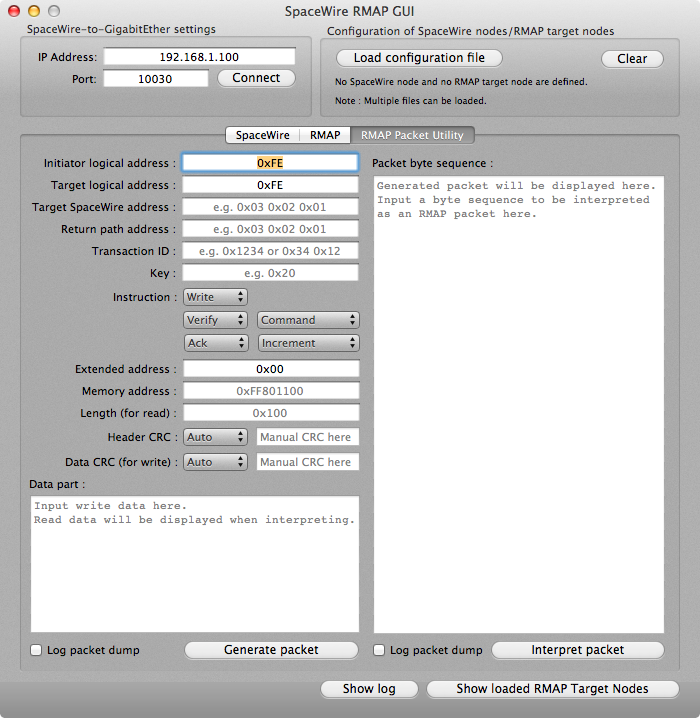
\includegraphics[width=8cm]{figures/SpaceWireRMAPGUI/Screenshot_RMAPPacketUtilityTab.png}
\caption{Screenshot of the RMAP Packet Utility tab.}
\label{figure:RMAPPacketUtilityTab}
\end{center}
\end{minipage}
\end{center}
\end{figure}


\subsection{Log message window}
The software displays log messages when a user executes each function.
Log messages are tagged with real time, and colored when there happens any error or unexpected event.
Users can open the log window, as shown in Figure \ref{figure:LogWindow} by clicking the "Show log" button in the bottom of the main window.

\subsection{Registered RMAP Target Nodes window}
When loading a configuration file, information of RMAP Target Nodes such as target logical address, key, and so on, are registered, and available with identifiers, or name, of the target.
The Registered RMAP Target Nodes window lists registered RMAP Target Nodes and their properties including defined those of memory objects.
Figure \ref{figure:RegisteredRMAPTargetNodesWhenLoadingConfigurationFile} shows an example of the window when loading a sample XML file for the SpaceWire-to-GigabitEther configuration port.

\begin{figure}[htb]
\begin{center}
\begin{minipage}{0.45\hsize}
\begin{center}
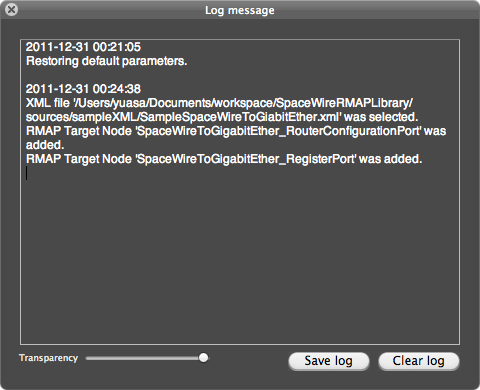
\includegraphics[width=8cm]{figures/SpaceWireRMAPGUI/Screenshot_LogWhenLoadingConfigurationFile.png}
\caption{Screenshot of the log window.}
\label{figure:LogWindow}
\end{center}
\end{minipage}
\hspace{0.05\hsize}
\begin{minipage}{0.45\hsize}
\begin{center}
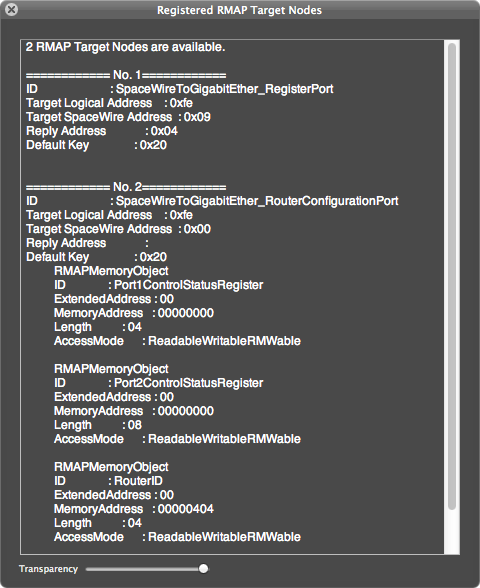
\includegraphics[width=8cm]{figures/SpaceWireRMAPGUI/Screenshot_RegisteredRMAPTargetNodesWhenLoadingConfigurationFile.png}
\caption{Screenshot of the Registered RMAP Target Nodes window.}
\label{figure:RegisteredRMAPTargetNodesWhenLoadingConfigurationFile}
\end{center}
\end{minipage}
\end{center}
\end{figure}


\subsection{Typical procedure}
When analyzing/creating RMAP packets in the RMAP Packet Utility tab, no connection to SpaceWire-to-GigabitEther is necessary.
When sending/receiving SpaceWire packets or initiating RMAP read/write, follow the procedure below:
\begin{enumerate}
  \setlength{\parskip}{0cm}
  \setlength{\itemsep}{0cm}
\item Set the IP address and the TCP port number.
\item Click the "Connect" button.
\item Load XML configuration files (to register RMAP Target Node information) if needed.
\item Send/receive SpaceWire packets (from the SpaceWire tab), \\
or initiate RMAP read/write (from the RMAP tab).\\
\end{enumerate}

\subsection{Notation of byte sequence}\label{section:numberNotation}
In SpaceWire RMAP GUI, users are required to input values (e.g. RMAP memory address and transaction ID) and 
byte sequence (e.g. raw SpaceWire packet and SpaceWire address).

The software interprets a value as hex when a leading "0x" is attached to numbers (and a-f).
Multi-byte numbers can be expressed as for example "0x1234abcd", and this example is interpreted as a byte sequence "0x12 0x34 0xab 0xcd".
When converting a multi-byte number with an odd number of digits e.g. "0x123" to a byte sequence, one leading 0 is padded, resulting "0x0123" == "0x01 0x23".

Numbers with no "0x" prefix are basically treated as decimal, but when the "All hex" option which is available in a part of input fields is enabled, "0x" is automatically put before the numbers. For example, "0x45 12 ab 0x88 f0" is converted to a byte sequence "0x45 0x12 0xab 0x88" when the "All hex" option is enabled.


%%%%%%%%%%%%%%%%%%%%%%%%%%%%%%%%%%%%%%
%%%%%%%%%%%%%%%%%%%%%%%%%%%%%%%%%%%%%%
\section{Settings}
\subsection{TCP/IP connection to SpaceWire-to-GigabitEther}\label{section:setting_section}
SpaceWire RMAP GUI should be used with SpaceWire-to-GigabitEther which provides a physical connection to SpaceWire network via TCP/IP over GigabitEthernet. The device can be purchased from Shimafuji Electric as a paid product, or an open-source (free) version on commercial FPGA board (ZestET1 by OrangeTree) is available from the open-source SpaceWire project.

Users can set an IP address (or URL) and utilized port number of SpaceWire-to-GigabitEther in the section on top-left of the main window as shown in Figure \ref{figure:section_SpaceWire-to-GigabitEther}. When the "Connect" button is clicked, the software tries to connect to the specified SpaceWire-to-GigabitEther, and then SpaceWire packet sending/receiving and RMAP initiator functions become available if a connection is successfully established. If timeout occurs, an error dialog will be displayed.

\begin{figure}[htb]
\begin{center}
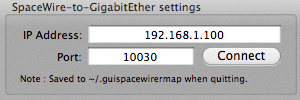
\includegraphics[height=2.5cm]{figures/SpaceWireRMAPGUI/Section_SpaceWire-to-GigabitEther_settings.png}
\caption{Input files for the IP address and the TCP port number of SpaceWire-to-GigabitEther.}
\label{figure:section_SpaceWire-to-GigabitEther}
\end{center}
\end{figure}

Note: Port number selects SpaceWire port of the internal SpaceWire router (when available on your SpaceWire-to-GigabitEther device). The default value 10030 may correspond to port 6 in Shimafuji's SpaceWire-to-GigabitEther, and port 1 in open-source SpaceWire-to-GigabitEther (which does not implement an internal router, and the port is directly connected to the physical connector on the board). For details, please refer to user guide of your SpaceWire-to-GigabitEther.

\subsection{RMAP Target Node definition using XML-like files}\label{section:configuration_section}
In SpaceWire RMAP GUI, an XML-like text file or files is/are used to load RMAP target node information such as a logical address, target SpaceWire address and reply address, and memory object (or register) information on the RMAP target node such as memory address, access length, access modes. This allows users to deal  with a large network which consists of large number of RMAP target nodes by avoiding manual reconfiguration of many input fields in the RMAP tab in every RMAP access.

The example shown below tells typical syntax used to define an RMAP Target Node and memory objects on it.  See SpaceWire/RMAPLibrary User Guide for details of the format.

\begin{lstlisting}[label=source:xml_configurationfile_example, caption=An example of an XML-like configuration file.]
<root>

<RMAPTargetNode id="SpaceWireToGigabitEther_RouterConfigurationPort">
	<TargetLogicalAddress>0xFE</TargetLogicalAddress>
	<TargetSpaceWireAddress>0x00</TargetSpaceWireAddress>
	<ReplyAddress></ReplyAddress>
	<Key>0x20</Key>

	<RMAPMemoryObject id="Port1ControlStatusRegister">
		<ExtendedAddress>0x00</ExtendedAddress>
		<Address>0x0000</Address>
		<Length>0x04</Length>
		<Key>0x20</Key>
	</RMAPMemoryObject>

	<RMAPMemoryObject id="Port2ControlStatusRegister">
		<ExtendedAddress>0x00</ExtendedAddress>
		<Address>0x0000</Address>
		<Length>0x08</Length>
		<Key>0x20</Key>
	</RMAPMemoryObject>

	<RMAPMemoryObject id="RouterID">
		<ExtendedAddress>0x00</ExtendedAddress>
		<Address>0x404</Address>
		<Length>0x04</Length>
		<Key>0x20</Key>
	</RMAPMemoryObject>
</RMAPTargetNode>

<RMAPTargetNode id="SpaceWireToGigabitEther_RegisterPort">
	<TargetLogicalAddress>0xFE</TargetLogicalAddress>
	<TargetSpaceWireAddress>0x09</TargetSpaceWireAddress>
	<ReplyAddress>0x04</ReplyAddress>
	<Key>0x20</Key>	
</RMAPTargetNode>

</root>
\end{lstlisting}

By loading configuration files from the "Configuration" section in the main window which is shown in Figure \ref{figure:section_ConfigurationFiles}, defined RMAP Target Nodes will be listed in the pull-down menu in "Initiator and Target Information" section of the RMAP tab. When one of defined RMAP Target Node is selected, its information is automatically set to relevant input fields, and correspondingly memory objects will be displayed in the register name pull-down menu in the "Memory Information" section. When selecting an entry from the register name pull-down menu, memory address and length will be automatically set.
\begin{figure}[htb]
\begin{center}
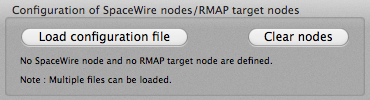
\includegraphics[height=2.5cm]{figures/SpaceWireRMAPGUI/Section_LoadConfigurationFile.png}
\vspace{-2mm}
\caption{Configuration file section.}
\label{figure:section_ConfigurationFiles}
\end{center}
\end{figure}

The above example results with RMAP Target Nodes named "SpaceWireToGigabitEther\_RouterConfigurationPort" and "SpaceWireToGigabitEther\_RegisterPort", and memory objects on "SpaceWireToGigabitEther\_RouterConfigurationPort" named "Port1ControlStatusRegister", "Port2ControlStatusRegister", and "RouterID" each having 4-byte fields. Figure \ref{figure:section_pull-down_menus} shows a screenshot of the RMAP Target Node pull-down menu and the register pull-down menu in the RMAP tab after loading the configuration file.
\begin{figure}[htb]
\begin{center}
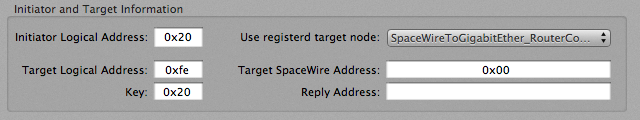
\includegraphics[height=2.5cm]{figures/SpaceWireRMAPGUI/Section_InitiatorAndTargetInformation_with_registered_RMAPTargetNode.png}\\\vspace{2mm}
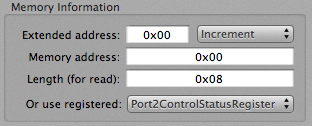
\includegraphics[height=2.5cm]{figures/SpaceWireRMAPGUI/Section_MemoryInformation_with_registered_MemoryObject.png}
\caption{The Initiator and Target Information section (top) and the Memory Information section (bottom) after loading the example XML configuration file, and selecting one of the defined entries in each pull-down menu.}
\label{figure:section_pull-down_menus}
\end{center}
\end{figure}



%%%%%%%%%%%%%%%%%%%%%%%%%%%%%%%%%%%%%%
%%%%%%%%%%%%%%%%%%%%%%%%%%%%%%%%%%%%%%
\section{SpaceWire functions}
\subsection{Sending packets}
To send packets, input byte sequence in the Raw Packet Send section on the SpaceWire window.
Figure \ref{figure:SpaceWireSection_RawPacketSend_withData} shows an example of data input.
See \S\ref{section:numberNotation} for details of number input options. Input byte sequence is sent with an end-of-packet marker, EOP or EEP, selected via "Send with EOP" or "Send with EEP".

\begin{figure}[htb]
\begin{center}
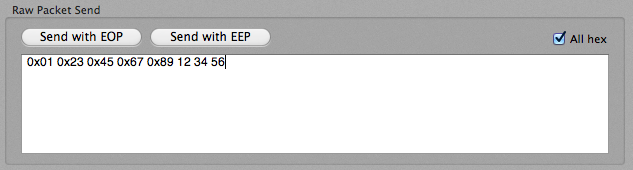
\includegraphics[width=10cm]{figures/SpaceWireRMAPGUI/SpaceWireSection_RawPacketSend_withData.png}
\vspace{-2mm}
\caption{An example of sending a packet.}
\label{figure:SpaceWireSection_RawPacketSend_withData}
\end{center}
\end{figure}


\subsection{Receiving packets}
To receive a packet as a raw SpaceWire packet, click "Receive (1 packet)". When a packet is received within a timeout duration which is set via the "Receive timeout" field (in units of milli second), its byte sequence is displayed in the text field.

Multiple packets can be continuously received, by clicking "Receive (continuous)".
When many packets are received in a short time, only a part of them is displayed. 

Note: To receive packets in the SpaceWire tab, the RMAPEngine used in the RMAP tab should be stopped because RMAPEngine tries to receive all incoming packets in background disabling packet receiving of the SpaceWire tab (this is caused by the two tabs shares one physical SpaceWire connection).


\begin{figure}[htb]
\begin{center}
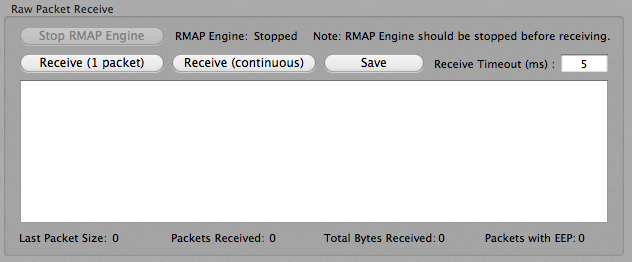
\includegraphics[width=10cm]{figures/SpaceWireRMAPGUI/SpaceWireSection_RawPacketReceiveSection.png}
\vspace{-2mm}
\caption{The Raw Packet Receive window.}
\label{figure:SpaceWireSection_RawPacketReceiveSection}
\end{center}
\end{figure}



\subsection{Emitting timecode}
Timecode character can be emitted by clicking "Emit one-shot" or "Emit periodically".
One-shot emission uses timecode value in the Timecode value field.
During periodic timecode emission, timecode value is automatically incremented, and emitted at a rate specified in the Timecode frequency field in units of Hz. Too low or too high timecode frequency results an error message to prevent from unexpected response of SpaceWire-to-GigabitEther and connected SpaceWire nodes. Current timecode value, and periodic emission status is displayed in the left part of the timecode section.

\begin{figure}[htb]
\begin{center}
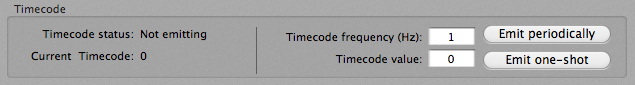
\includegraphics[width=10cm]{figures/SpaceWireRMAPGUI/SpaceWireSection_TimecodeSection.png}
\vspace{-2mm}
\caption{Timecode section in the SpaceWire tab.}
\label{figure:SpaceWireSection_TimecodeSection}
\end{center}
\end{figure}


%%%%%%%%%%%%%%%%%%%%%%%%%%%%%%%%%%%%%%
%%%%%%%%%%%%%%%%%%%%%%%%%%%%%%%%%%%%%%
\section{RMAP functions}
To perform RMAP read/write, various types of information must be provided; information of an RMAP target node (i.e. destination of an RMAP command packet), memory information (i.e. address and length), instruction (i.e. read or write with verify/no verify and/or reply/no reply), and information regarding a transaction (transaction ID mode and timeout duration).

Figure \ref{figure:RMAPSection_InitiatorAndTargetInformation} shows  the Initiator and Target information section, whose content can be manually input, or registered RMAP Target Node information can be loaded from the Use registered target node pull-down menu. Note that the target node address field accepts inputs like "0x03 0x0f" and "0x030f" as well. When an input reply address has a length which is not a multiple of 4, leading 0s are automatically padded.

\begin{figure}[htb]
\begin{center}
\begin{minipage}[t]{0.45\hsize}
\begin{center}
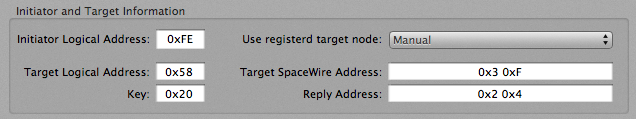
\includegraphics[width=8.3cm]{figures/SpaceWireRMAPGUI/RMAPSection_InitiatorAndTargetInformation.png}
\vspace{-2mm}
\caption{The Initiator and Target information section. Target SpaceWire address and Reply address are interpreted as "0x03 0x0f" and "0x00 0x00 0x02 0x04" in this example.}
\label{figure:RMAPSection_InitiatorAndTargetInformation}
\end{center}
\end{minipage}
\hspace{0.05\hsize}
\begin{minipage}[t]{0.45\hsize}
\begin{center}
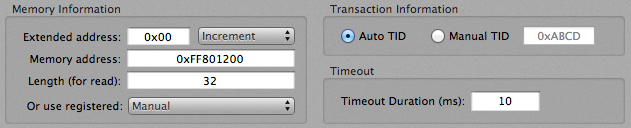
\includegraphics[width=8.3cm]{figures/SpaceWireRMAPGUI/RMAPSection_MemoryTransactionIDTimeoutInformation.png}
\vspace{-2mm}
\caption{The Memory, the transaction ID, and the timeout sections.}
\label{figure:RMAPSection_MemoryTransactionIDTimeoutInformation}
\end{center}
\end{minipage}
\end{center}
\end{figure}


Refer specifications or user manuals of RMAP target devices for memory addresses accessible via RMAP.
Length is only necessary for read transactions, and is automatically calculated for write transactions.

Transaction management is done by the internal RMAP Engine based on transaction ID.
Although automatic transaction ID assignment, which is default of SpaceWire RMAP GUI, will be acceptable for many use cases, users can also specify a transaction ID manually to force the RMAP Engine to put the transaction ID to an RMAP command packet.
When using a manually selected transaction ID, please carefully check if an emitted RMAP command packet has an expected transaction ID (e.g. by checking "Log packet dump").

\subsection{Performing Write and Read}
After setting the initiator and the target information and the memory information, users can perform RMAP write and read very easily. Figure \ref{figure:RMAPSection_Write} shows the write data section with an example write data. Clicking "RMAP Write", an RMAP Write command packet will be sent to a designated target node. In RMAP Write, the data length is automatically calculated from the input data, and the length field is ignored. Whether a user request verification on data (i.e. CRC calculation) and/or a reply for the command packet can be selected from the Options field. When a reply is not received within a specified timeout duration although it (a reply) is requested, an error message will be reported in the log window. Users can input multi-byte data like 0xabcdef1234, and this is treated as an array of 0xab 0xcd 0xef 0x12 0x34 (see \S\ref{section:numberNotation}).

In RMAP Read, read length should be specified in the length field (in the Memory information section above). By clicking "RMAP Read", an RMAP Read command packet is sent to a target node. When a reply packet is received within a timeout duration, read data will be displayed in the RMAP Read section (byte-to-byte) as shown in Figure \ref{figure:RMAPSection_Read}. Timeout is logged as an error message.

\begin{figure}[htb]
\begin{center}
\begin{minipage}[t]{0.45\hsize}
\begin{center}
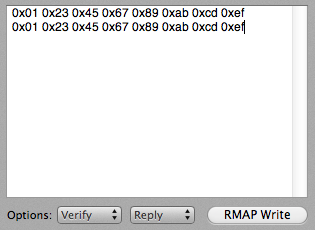
\includegraphics[width=7cm]{figures/SpaceWireRMAPGUI/RMAPSection_Write.png}
\vspace{-2mm}
\caption{The RMAP Write section with write data.}
\label{figure:RMAPSection_Write}
\end{center}
\end{minipage}
\hspace{0.05\hsize}
\begin{minipage}[t]{0.45\hsize}
\begin{center}
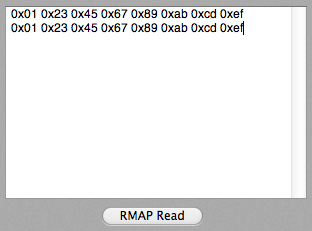
\includegraphics[width=7cm]{figures/SpaceWireRMAPGUI/RMAPSection_Read.png}
\vspace{-2mm}
\caption{The RMAP Read section with read data.}
\label{figure:RMAPSection_Read}
\end{center}
\end{minipage}
\end{center}
\end{figure}


\subsection{Errors and timeout}
When an RMAP reply packet with a status other than "Command Successfully Executed (0x00)", an error message is reported in the log window. Timeout is also reported as an error with a message shown in Figure \ref{figure:RMAPSection_ReadTimeout}. 

\begin{figure}[htb]
\begin{center}
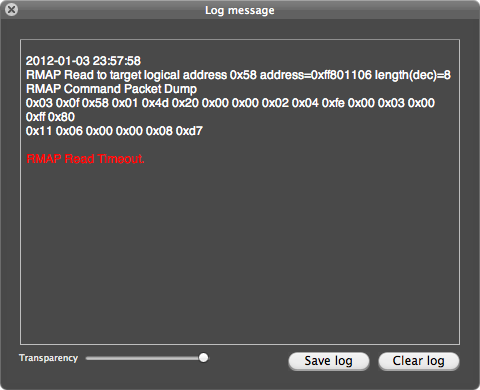
\includegraphics[width=8cm]{figures/SpaceWireRMAPGUI/RMAPSection_ReadTimeout.png}
\vspace{-2mm}
\caption{Timeout message reported in the log window.}
\label{figure:RMAPSection_ReadTimeout}
\end{center}
\end{figure}


\subsection{Use defined RMAP Target Nodes and memory objects}
After loading an XML-like configuration file (\S\ref{section:configuration_section}), users can use registered information of RMAP Target Nodes such as target logical address, reply address, memory address, data length, and so on.
Select a target node and its memory object from the "Use registered target node" and the "Use registered" pull-down menus, respectively. Registered information will be updated to corresponding fields.

To clear registered RMAP Target Node information, click "Clear nodes" in the Configuration section. Details of registered RMAP Target Nodes (text dump) are available from the sub window (click "Show registered RMAP Target Nodes").

\subsection{Logging dump of an RMAP packet}
By checking "Log packet dump" beneath the RMAP Read button, all the sent and received RMAP packets are logged so as to allow off-line analyses of the packets. Figure \ref{figure:RMAPSection_LogRMAPPacketDump} shows an example of logging a transaction, i.e. command and reply packets. Since SpaceWire RMAP GUI has an integrated RMAP packet analysis function in the RMAP Packet Utility tab, users can easily analyze packets by copying and pasting byte sequence to the tab, and then clicking "Interpret as an RMAP packet".

\begin{figure}[htb]
\begin{center}
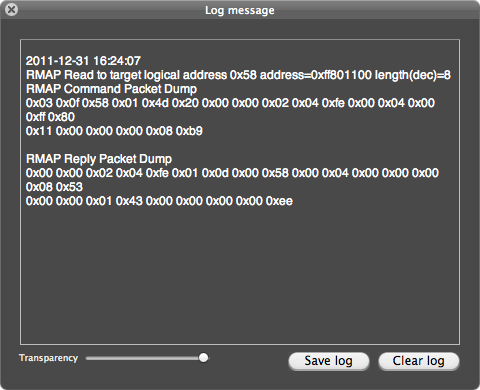
\includegraphics[width=8cm]{figures/SpaceWireRMAPGUI/RMAPSection_LogRMAPPacketDump.png}
\vspace{-2mm}
\caption{Logged RMAP packet dump.}
\label{figure:RMAPSection_LogRMAPPacketDump}
\end{center}
\end{figure}


%%%%%%%%%%%%%%%%%%%%%%%%%%%%%%%%%%%%%%
%%%%%%%%%%%%%%%%%%%%%%%%%%%%%%%%%%%%%%
\section{RMAP Packet Utility functions}
SpaceWire RMAP GUI provides capabilities of inspecting and constructing RMAP packets.
The RMAP Packet Utility tab is an interface to these functionalities.

\subsection{Creating RMAP packets}
When creating an RMAP packet, input properties of the packet, and then click "Generate packet".
Resulting packet byte sequence will be shown in the right text field.
Figure \ref{figure:RMAPPacketUtilitySection_GenerateInterpret} presents a result of generation of a packet shown in the RMAP standard document ("RMAP non-verified incrementing write-with-reply command - without SpaceWire addresses"; for see A.4 of the document).
By checking "Log dump packet", details of the generated packet is added as a log message as Figure \ref{figure:RMAPPacketUtilitySection_Log_Generate} shows.

\subsection{Interpreting RMAP packets}
Input byte sequence to the right text field, and then click "Interpret packet". Header information and data will be set to text fields in the left column. 
Like the generation function, detailed packet interpretation log can be displayed by checking "Log packet dump" next to the "Interpret packet" button.

\begin{figure}[htb]
\begin{center}
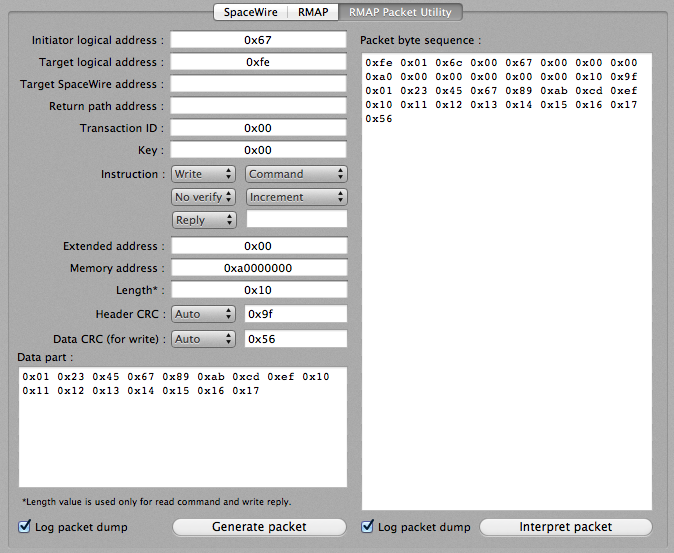
\includegraphics[width=10cm]{figures/SpaceWireRMAPGUI/RMAPPacketUtilitySection_GenerateInterpret.png}
\vspace{-2mm}
\caption{An example of RMAP packet generation/interpretation.}
\label{figure:RMAPPacketUtilitySection_GenerateInterpret}
\end{center}
\end{figure}

\begin{figure}[htb]
\begin{center}
\begin{minipage}[t]{0.45\hsize}
\begin{center}
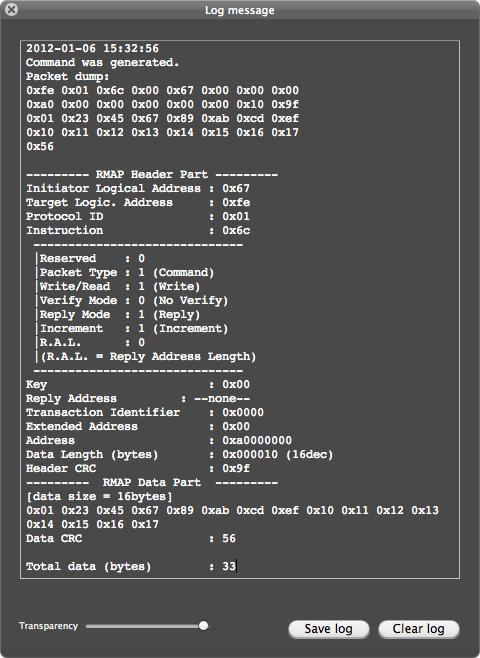
\includegraphics[width=8cm]{figures/SpaceWireRMAPGUI/RMAPPacketUtilitySection_Log_Generate.png}
\vspace{-2mm}
\caption{Log message added when generating an RMAP packet. Note that "Log packet button" is checked. }
\label{figure:RMAPPacketUtilitySection_Log_Generate}
\end{center}
\end{minipage}
\hspace{0.05\hsize}
\begin{minipage}[t]{0.45\hsize}
\begin{center}
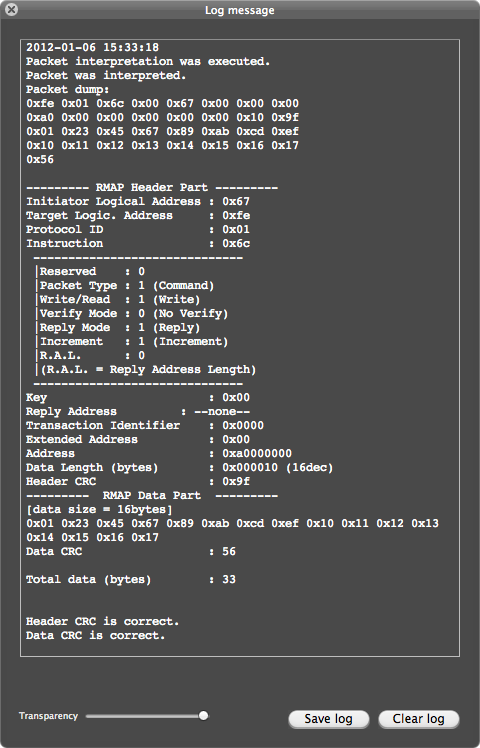
\includegraphics[width=8cm]{figures/SpaceWireRMAPGUI/RMAPPacketUtilitySection_Log_Interpret.png}
\vspace{-2mm}
\caption{Log message added when interpreting an RMAP packet. Note that "Log packet button" is checked. }
\label{figure:RMAPPacketUtilitySection_Log_Interpret}
\end{center}
\end{minipage}
\end{center}
\end{figure}


\subsection{CRC error}
The packet interpretation function reports a warning when it detects an invalid CRC in the header or the data as shown in Figures \ref{figure:RMAPPacketUtilitySection_Interpret_InvalidCRCs_01}, \ref{figure:RMAPPacketUtilitySection_Interpret_InvalidCRCs_02}, and \ref{figure:RMAPPacketUtilitySection_Interpret_InvalidCRCs_03}.
A correct CRC value is automatically calculated and set to the CRC field in the left column. The value is also displayed in the log window.


\begin{figure}[htb]
\begin{center}
\begin{minipage}[t]{0.45\hsize}
\begin{center}
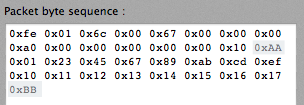
\includegraphics[width=6cm]{figures/SpaceWireRMAPGUI/RMAPPacketUtilitySection_Interpret_InvalidCRCs_01.png}
\vspace{-2mm}
\caption{Sample packet with invalid header and data CRCs (shaded bytes).}
\label{figure:RMAPPacketUtilitySection_Interpret_InvalidCRCs_01}
\end{center}
\end{minipage}
\hspace{0.05\hsize}
\begin{minipage}[t]{0.45\hsize}
\begin{center}

\includegraphics[width=6cm]{figures/SpaceWireRMAPGUI/RMAPPacketUtilitySection_Interpret_InvalidCRCs_02.png}
\vspace{-2mm}
\caption{Valid CRC values calculated in interpretation.}
\label{figure:RMAPPacketUtilitySection_Interpret_InvalidCRCs_02}
\end{center}
\end{minipage}
\end{center}
\end{figure}

\begin{figure}[htb]
\begin{center}
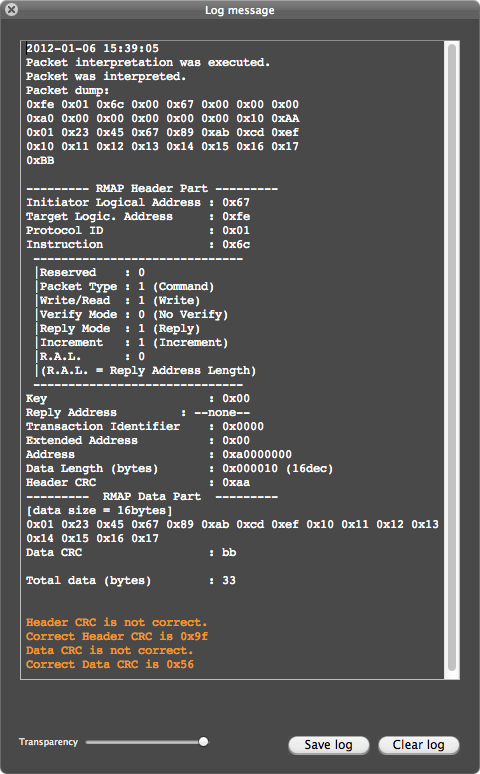
\includegraphics[width=8cm]{figures/SpaceWireRMAPGUI/RMAPPacketUtilitySection_Interpret_InvalidCRCs_03.png}
\vspace{-2mm}
\caption{Log message shown when interpreting the same packet shown in Figure \ref{figure:RMAPPacketUtilitySection_Interpret_InvalidCRCs_01}. Note the orange message telling CRCs are invalid.}
\label{figure:RMAPPacketUtilitySection_Interpret_InvalidCRCs_03}
\end{center}
\end{figure}


\clearpage

%%%%%%%%%%%%%%%%%%%%%%%%%%%%%%%%%%%%%%
%%%%%%%%%%%%%%%%%%%%%%%%%%%%%%%%%%%%%%
\appendix
\section{Format of the XML-like configuration file}
RMAP Target Node information and memory object information can be stored in an XML-like configuration file.
The format is defined in SpaceWire/RMAP Library, specifically, in the RMAPTargetNode class and the RMAPMemoryObject class, and therefore, for details, see SpaceWire/RMAP Library User Guide.

Structures of RMAPTargetNode and RMAPMemoryObject are listed below. When one (or more) of mandatory tag is not found, the configuration file is discarded.
\begin{description}
  \setlength{\parskip}{0cm}
  \setlength{\itemsep}{0cm}
\item[RMAPTargetNode] id (name) attribute is mandatory.
	\begin{description}
	  \setlength{\parskip}{0cm}
	  \setlength{\itemsep}{0cm}
	  \item[TargetLogicalAddress] Mandatory.
	  \item[TargetSpaceWireAddress] Mandatory. Array of 0x00-0xFF. (e.g.  0x02 0x0a 0x07 0x01)
	  \item[ReplyAddress] Mandatory. Array of 0x00-0xFF. (e.g.  0x02 0x0a 0x07 0x01)
	  \item[Key] Mandatory. 0x00-0xFF.
	  \item[InitiatorLogicalAddress] Optional. 0x00-0xFF.
	\end{description}	  
\item[RMAPMemoryObject] id (name) attribute is mandatory.
	\begin{description}
	  \setlength{\parskip}{0cm}
	  \setlength{\itemsep}{0cm}
	  \item[ExtendedAddress] Optional. Default is 0x00.
	  \item[Address] Mandatory. 0x00000000-0xFFFFFFFF.
	  \item[Length] Mandatory. 0x000000-0xFFFFFF.
	  \item[Key] Optional. 0x00-0xFF. The value defined in the parent RMAPTargetNode is overridden by this value if set.
	  \item[AccessMode] Optional. Any of ReadWrite, ReadOnly, WriteOnly, Readable (=ReadOnly), Writable (=WriteOnly).
	  \item[IncrementMode] Optional. Either of Increment or NoIncrement.
	\end{description}	  
\end{description}
The below shows a template for a configuration file.
Note that one file can contain multiple RMAPTargetNodes, and one RMAPTargetNode tag can contains multiple memory object definitions.
\begin{lstlisting}[label=source:xml_configurationfile_template, caption=Tags which define RMAPTargetNode and RMAPMemoryObject.]
<root>

<RMAPTargetNode id="NameOfTheRMAPTargetNode">
	<TargetLogicalAddress>0xFE</TargetLogicalAddress>
	<TargetSpaceWireAddress>0x00</TargetSpaceWireAddress>
	<ReplyAddress></ReplyAddress>
	<Key>0x20</Key>
	<InitiatorLogicalAddress>0x35</InitiatorLogicalAddress>	<!-- optional -->
	
	<RMAPMemoryObject id="NameOfTheMemoryObjectOnTheRMAPTargetNode">
		<ExtendedAddress>0x00</ExtendedAddress>
		<Address>0x0000</Address>
		<Length>0x04</Length>
		<Key>0x20</Key>	<!-- optional -->
		<IncrementMode>Increment</IncrementMode>
	</RMAPMemoryObject>
	
	... other RMAPMemoryObject tags ...

</RMAPTargetNode>

... other RMAPTargetNode tags ...

</root>
\end{lstlisting}


\end{document}